\section{Heat of Vaporization of Nitrogen}

\begin{comment}
  Comment by Matt Trawick:
  In one of my 132 classes, when I had used the previous (more cook-booky)
  version of this lab, I put a problem on an exam where I just gave students
  a graph of weight vs. time for liquid nitrogen (part with heater on, part
  with heater off, each with a different slope) and told them the current and
  voltage of the heater, and  asked them to calculate the heat of vaporization.

  Exactly 3 students out of 24 could do it.

  So the next year I wrote a version of this lab, with many fewer
  directions, basically making them figure out for themselves what to
  do (presumably with some help from me when they got unstuck).  I put
  the same question on a different exam and 16 out of 20 students could
  do it (scoring 9 out of 10 points on the problem or above.) Based on
  that data, I conclude that this more minimimalist version of this
  lab is more effective.
\end{comment}

\makelabheader %(Space for student name, etc., defined in master.tex)

\bigskip

\textbf{Objective}

To measure the heat of vaporization of nitrogen.

\begin{wrapfigure}[6]{r}{0.49\textwidth}
    \vspace{0.1in}
    \includegraphics[width=0.49\textwidth]{latent_heat_of_vaporization_of_nitrogen/heat_vap_nit_fig_1.eps}
\end{wrapfigure}

\bigskip

\textbf{Apparatus}
\begin{itemize}
\item Force probe (with calibration weights)
\item Lab stand
\item Styrofoam cup
\item Liquid nitrogen
\item Power resistor
\item Power supply
\item Digital multimeter
  % 5/18/2015: Added the DMM back in.  Although the DMM is not strictly necessary (since our power supplies have current and voltage measurement on them) students should have a DMM in case they want to measure resistance or trouble-shoot something.
\item Wires
\item \textit{DataStudio} Software (\texttt{LiquidNitrogenVapor.ds})
\end{itemize}
%\vspace{0.3cm}
%{\raggedleft \resizebox*{0.5\textwidth}{!}{\includegraphics{heat_vap_nit_fig_1.eps}} \par}
%\usepackage{wrapfig}
%\resizebox*{0.5\textwidth}{!}{\includegraphics{heat_vap_nit_fig_1.eps}} \par}
%\vspace{0.3cm}

Your task is to measure the latent heat of vaporization for nitrogen with the equipment given.
Your basic strategy will be to use a resistor ``heater'' to put a known amount of thermal
energy into a container of liquid nitrogen, and to simultaneously use a force probe to
measure the amount of nitrogen changed from a liquid into a gas.

Some points to keep in mind:

\begin{enumerate}

\item You can measure three quantities that can help you find the power
dissipated in the resistor: $I$, $V$, and $R$. Be aware that the ``$\!R\,$'' may change drastically with temperature.

\item Some liquid nitrogen will boil away even with your heater turned off, just due to lousy thermal insulation. You'll have to account for this somehow.

\item Check your force measurements with known weights to make sure your force probe is properly calibrated and not giving completely bogus results.  (To calibrate your force probe, see Appendix \ref{datastudio}.) 

\item You will probably have to assume that the nitrogen gas given off is at exactly the same temperature as the liquid, even though it could be slightly hotter. Can you think of some good ways to either minimize this problem or account for it somehow?

\item Yes, you will need to estimate your uncertainty for this experiment. Does the accepted value for the latent heat of nitrogen fall within the range of your uncertainty?

\end{enumerate}

Good Luck!  :-)
